% ============================================================
% SmartQ — Smart Hospital Queue Management \& AI Triage System
% Detailed Academic Project Report (LaTeX for Overleaf)
% ============================================================
\documentclass[12pt,a4paper]{article}

% ─── Packages ───────────────────────────────────────────────
\usepackage[utf8]{inputenc}
\usepackage[T1]{fontenc}
\usepackage{lmodern}
\usepackage[margin=1in]{geometry}
\usepackage{graphicx}
\usepackage{booktabs}
\usepackage{longtable}
\usepackage{array}
\usepackage{tabularx}
\usepackage{multirow}
\usepackage{enumitem}
\usepackage{amsmath}
\usepackage{hyperref}
\usepackage{xcolor}
\usepackage{listings}
\usepackage{tikz}
\usepackage{float}
\usepackage{caption}
\usepackage{subcaption}
\usepackage{fancyhdr}
\usepackage{titlesec}
\usepackage{setspace}
\usepackage[ruled,vlined,linesnumbered]{algorithm2e}
\usepackage{tocloft}

\usetikzlibrary{shapes.geometric, arrows.meta, positioning, fit, backgrounds, calc}

% ─── Hyperref Setup ─────────────────────────────────────────
\hypersetup{
    colorlinks=true,
    linkcolor=blue!70!black,
    citecolor=blue!70!black,
    urlcolor=blue!70!black,
    bookmarksnumbered=true,
    pdfauthor={},
    pdftitle={SmartQ — Smart Hospital Queue Management \& AI Triage System},
    pdfsubject={MADLAB Project Report},
}

% ─── Code Listing Style ─────────────────────────────────────
\definecolor{codebg}{RGB}{248,248,248}
\definecolor{codegreen}{RGB}{0,128,0}
\definecolor{codegray}{RGB}{128,128,128}
\definecolor{codeblue}{RGB}{0,0,180}
\definecolor{codepurple}{RGB}{128,0,128}

\lstdefinestyle{mystyle}{
    backgroundcolor=\color{codebg},
    basicstyle=\ttfamily\footnotesize,
    breakatwhitespace=false,
    breaklines=true,
    captionpos=b,
    commentstyle=\color{codegreen},
    keywordstyle=\color{codeblue}\bfseries,
    numberstyle=\tiny\color{codegray},
    stringstyle=\color{codepurple},
    showstringspaces=false,
    numbers=left,
    numbersep=8pt,
    frame=single,
    rulecolor=\color{black!30},
    tabsize=2,
    xleftmargin=15pt,
    framexleftmargin=15pt,
}
\lstset{style=mystyle}

% ─── Pseudocode listing style ───────────────────────────────
\lstdefinestyle{pseudo}{
    backgroundcolor=\color{codebg},
    basicstyle=\ttfamily\footnotesize,
    breaklines=true,
    frame=single,
    rulecolor=\color{black!30},
    xleftmargin=15pt,
    framexleftmargin=15pt,
    numbers=none,
    showstringspaces=false,
    mathescape=true,
    morekeywords={FUNCTION, IF, THEN, RETURN, ELSE, FOR, WHILE, END, SET, PUSH, REMOVE, UPDATE, FIND, ORDER, BY, ASC, AND, OR, WHERE, SAVE, REJECT, MAX, ROUND, SUM, LENGTH, INDEX, PREDICT, AWAIT},
    keywordstyle=\color{codeblue}\bfseries,
}

% ─── Section Formatting ─────────────────────────────────────
\titleformat{\section}{\large\bfseries\sffamily}{\thesection.}{0.5em}{}
\titleformat{\subsection}{\normalsize\bfseries\sffamily}{\thesubsection}{0.5em}{}
\titleformat{\subsubsection}{\normalsize\itshape\sffamily}{\thesubsubsection}{0.5em}{}

% ─── Header / Footer ────────────────────────────────────────
\pagestyle{fancy}
\fancyhf{}
\fancyhead[L]{\small\textit{SmartQ — Smart Hospital Queue \& AI Triage}}
\fancyhead[R]{\small\textit{MADLAB Project Report}}
\fancyfoot[C]{\thepage}
\renewcommand{\headrulewidth}{0.4pt}
\renewcommand{\footrulewidth}{0pt}

% ─── Spacing ─────────────────────────────────────────────────
\setstretch{1.25}

% ─── Custom Commands ─────────────────────────────────────────
\newcommand{\cmark}{\textcolor{green!60!black}{\checkmark}}
\newcommand{\xmark}{\textcolor{red!70!black}{$\times$}}
\newcommand{\dash}{---}

% ============================================================
\begin{document}

% ─── Title Page ──────────────────────────────────────────────
\begin{titlepage}
    \centering
    \vspace*{2cm}
    
    {\Huge\bfseries\sffamily SmartQ}\\[0.5cm]
    {\LARGE\sffamily Smart Hospital Queue Management \& AI Triage System}\\[2cm]
    
    {\Large\textbf{Comprehensive Project Report}}\\[0.5cm]
    {\large MADLAB Project — Semester 6}\\[3cm]
    
    \rule{0.6\textwidth}{0.4pt}\\[1cm]
    
    {\Large\textbf{Team Members}}\\[0.5cm]
    {\large
    \begin{tabular}{l@{\hspace{1.5cm}}r}
        Utkarsh Jha & 230953422 \\[0.3cm]
        Mihir Sahay & 230953498 \\[0.3cm]
        Rishi Khandelwal & 230953494 \\[0.3cm]
        Omkar Nayak & 230953502 \\
    \end{tabular}
    }\\[1.5cm]
    
    {\large
    \begin{tabular}{rl}
        \textbf{Subject:} & Mobile Application Development Laboratory \\[0.3cm]
        \textbf{Academic Year:} & 2025--2026 \\
    \end{tabular}
    }
    
    \vfill
    
    {\large\today}
\end{titlepage}

% ─── Table of Contents ──────────────────────────────────────
\newpage
\tableofcontents
\newpage

% ============================================================
% ABSTRACT
% ============================================================
\section*{Abstract}
\addcontentsline{toc}{section}{Abstract}

The outpatient department (OPD) of any hospital is the primary access point to specialized healthcare. Historically, this phase is plagued by extreme congestion, disorganization, an inability to prioritize serious conditions properly, and patient dissatisfaction due to immense waiting times with zero visibility. While modernization has brought digitized kiosks to hospitals, these mere number-dispensers do nothing to triage urgency or interactively inform waiting patients. Our project, \textbf{SmartQ}, is an end-to-end cloud-synchronized, AI-augmented queue and triage platform that solves this fundamental bottleneck.

SmartQ provides a robust \textbf{triple-tier architecture}: a Material Design-compliant native Android frontend utilizing biometric authentication; a Node.js/Express.js RESTful API managing state synchronization and dynamic ETA computations; and a FastAPI Machine Learning Service exposing the production triage predictor together with rule-assisted specialty routing, safety checks, and test recommendation helpers.

The application removes the need for physical hospital kiosks. Patients can onboard from home, describe their symptoms in natural language, and let SmartQ combine model-backed KTAS prediction with rule-assisted specialty routing, safety flag detection, and suggested baseline tests. This triage output combines dynamically with visit context to re-order the queue using a priority-aware insertion algorithm, pushing high-priority and safety-sensitive patients toward faster review. To assist patient agency, SmartQ allows patients to 'snooze' their turn if caught in traffic, track a live-updating moving-average ETA, and log securely using Fingerprint/FaceID credentials. Administrators, nurses, and doctors receive specialized dashboards allowing total command over hospital flow logic. This report documents the implemented architecture, operational logic, database structure, and the exact machine learning metrics of the deployed system.

\vspace{0.5em}
\noindent\textbf{Keywords:} Artificial Intelligence Clinical Triage, Fast Queue Management System, Native Android Application, XGBoost, Priority Scheduling, FastAPI, REST API, MongoDB, Biometric Security, Machine Learning Inference.

\newpage

% ============================================================
% 1. INTRODUCTION
% ============================================================
\section{Introduction}

The healthcare infrastructures of densely populated environments face an inherently asymmetric relationship: the volumetric flow of patients seeking diagnostics dramatically outweighs the available practitioner hours. Within the Outpatient Department (OPD), this disparity results in overcrowded waiting areas, immense patient anxiety, cross-infection risks, and severely long unmanaged waiting times. The psychological element of waiting is exacerbated when patients have no estimated time of arrival (ETA), leaving them trapped out of fear of missing their turn. Consequentially, patients often surrender and exit the facility—a metric medically defined as "Left Without Being Seen" (LWBS).

The second major crisis within these departments is triaging. Traditional physical token dispensers operate on a rigid First-Come-First-Serve (FCFS) basis. Under FCFS, an 80-year-old patient suffering from acute angina who arrived at 9:05 AM is slotted behind a healthy 20-year-old seeking routine dermatological consultation who arrived at 9:02 AM. Without intervention from overburdened nursing staff, the rigid numeric system directly endangers the critical patient.

\textbf{SmartQ} fundamentally restructures this dynamic. By displacing the token acquisition phase from a physical kiosk into the patient's smartphone, we eliminate physical crowding immediately. Our primary contribution is integrating \textbf{clinical decision support} directly into the onboarding stream. Rather than trusting patients to navigate complex hospital routing correctly, they define their complaint natively (e.g. "My chest hurts really bad and I can't catch my breath when I lie down"). The FastAPI inference layer combines a saved XGBoost triage bundle, structured feature defaults, symptom normalization, and explicit safety rules. In practice, this allows SmartQ to estimate a KTAS (Korean Triage and Acuity Scale) priority band, surface confidence, suggest a route, and escalate obvious red flags such as respiratory distress or stroke-like symptoms for immediate review.

The system interacts robustly across three roles:
\begin{itemize}
    \item \textbf{Patients} securely log in utilizing Android Biometrics, acquire AI-triaged queue positions, track dynamic moving-average ETAs, and possess the agency to 'Snooze' (defer) their turn twice.
    \item \textbf{Doctors} obtain real-time dashboards mapping their exact caseload, allowing them to advance the queue via single taps, observing both symptoms and AI-recommended baseline tests.
    \item \textbf{Administrators} gain total oversight capabilities, possessing tools to compact queues (remove no-shows), pause queues during emergencies, view extensive hospital flow metrics, and trigger a bespoke ML Evaluation Suite to trace model outputs natively via a dedicated graphical tool.
\end{itemize}

% ============================================================
% 2. LITERATURE SURVEY
% ============================================================
\section{Literature Survey}

The theoretical foundation of SmartQ derives from intersecting studies in healthcare informatics, mobile engineering, and classical machine learning methodologies.

\subsection{Queue Management and Operations Research}
Haq et al. (2020) demonstrated that mobile-augmented smart queue systems dramatically reduce perceived waiting times by allowing patients to track queues off-premises. However, their system utilized generic allocation algorithms that could not differentiate patient severity. Konrad et al. (2017) utilized discrete event simulation modeling to prove mathematically that prioritizing high-acuity patients within standard queues significantly drastically reduces severe LWBS (Left Without Being Seen) rates without mathematically punishing lower-acuity patients to an intolerable degree. SmartQ operationalizes Konrad's simulation into a live software architecture.

\subsection{Machine Learning and Clinical Triage (KTAS Optimization)}
Standard symptom checkers have traditionally relied on rigid decision trees, which struggle with the nuance of human linguistics and the complex interaction of vital signs. While the industry has recently explored Transformer-based neural architectures (like BERT), these models often prove excessively heavy and prone to hallucination for strictly structured clinical tabular data (Age, SpO2, Heart Rate, BP). Research has shown that gradient boosting algorithms, specifically \textbf{XGBoost} (Chen \& Guestrin, 2016), frequently outperform deep neural networks on tabular clinical data classification tasks predicting 5-level acuity scales like the Emergency Severity Index (ESI) or KTAS. In SmartQ, this literature motivated the symptom-normalization and hybrid-routing design, where the deployed production stack uses a highly-tuned saved XGBoost triage bundle plus explicit safety and routing rules, enabling robust, low-latency, and highly explainable priority classification. 

\subsection{Authentication Security in mHealth}
As established by Soni et al. (2022), the security of RESTful APIs in mobile health heavily relies on stateless authentication mechanisms like JSON Web Tokens (JWT). While JWT handles the transport authorization flawlessly, securing the token on the physical device remains challenging resulting in potential credential theft. SmartQ solves this by implementing Android's \texttt{BiometricPrompt} framework, sealing standard login routines behind hardware-backed facial recognition and fingerprint modules mapped precisely to encrypted shared preferences.

% ============================================================
% 3. DETAILED OBJECTIVES
% ============================================================
\section{Detailed Objectives}

The project's execution is defined by highly specific functional and non-functional goals:

\begin{enumerate}
    \item \textbf{High-Fidelity Android Client Architecture}: Build a visually superior, native Java application utilizing complex XML abstractions (stitching methodologies), custom interpolator animations (scale, fade), and Material components.
    \item \textbf{FastAPI Machine Learning Inference Pipeline}: Deploy a Python FastAPI microservice that processes structured triage payloads alongside textual symptom descriptions through the saved XGBoost priority model, then augments the result with rule-assisted specialty routing, test suggestions, and critical safety-rule evaluations.
    \item \textbf{Robust Authentication via Biometrics}: Utilize bcrypt for backend password hashing, generate encrypted JWTs, and secure the Android application layer heavily utilizing hardware-level BiometricManager prompts mapping to the Android KeyStore.
    \item \textbf{Automated Queue Priority Triage}: Construct MongoDB aggregation pipelines and strictly atomic transaction blocks that seamlessly insert a high-priority patient (flagged by Age > 60 or by AI KTAS Severity 1/2) ahead of lower-priority users concurrently without raising race-conditions.
    \item \textbf{Dynamic Wait Time Predictions}: Abandon inaccurate static ETAs. Implement a backend mathematically-sound Simple Moving Average (SMA) calculating the last 10 exact consultation timelines to feed predictive ETAs live to the client via a 10-second polling handler.
    \item \textbf{Extensive Patient Agency}: Implement robust client logic to allow a 'Snooze' operation, safely bumping a patient back exact intervals (e.g., 2 slots) if they physically cannot arrive in time, bounded by a strict two-snooze algorithmic limit.
    \item \textbf{Supervisory Admin Controls}: Formulate an admin application screen capable of evaluating the AI model iteratively through a dashboard test-runner, purging 'no-shows' causing automatic queue compactions, and commanding hospital-wide queue pauses.
\end{enumerate}

% ============================================================
% 4. OVERALL SYSTEM ARCHITECTURE
% ============================================================
\section{Overall System Architecture}

SmartQ is built upon a fully decoupled, microservice-inspired cloud architecture. This physical separation prevents computationally expensive tasks (like DataFrame construction and Tree Boosting analysis) from blocking standard input/output operations necessary for lightning-fast UI responses.

\subsection{High-Level Architectural Diagram}

The system executes as a Microservice array illustrated in Figure \ref{fig:detailed_arch}.

\begin{figure}[H]
\centering
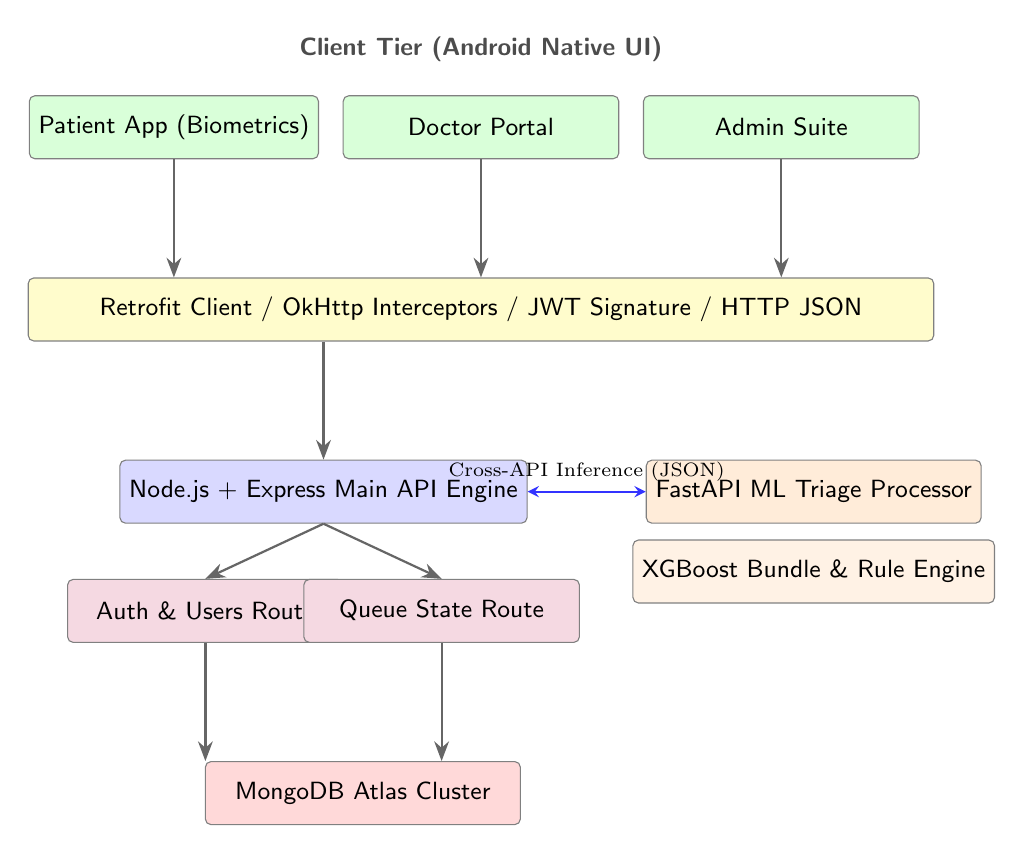
\begin{tikzpicture}[
    node distance=0.6cm,
    layer/.style={rectangle, draw=black!50, fill=#1, minimum width=3.5cm, minimum height=0.8cm, font=\small\sffamily, rounded corners=2pt},
    arrow/.style={-{Stealth[length=2.5mm]}, thick, draw=black!60},
    grouplabel/.style={font=\small\sffamily\bfseries, text=black!70}
]
    % Client Layer
    \node[layer=green!15] (patient) {Patient App (Biometrics)};
    \node[layer=green!15, right=0.3cm of patient] (docapp) {Doctor Portal};
    \node[layer=green!15, right=0.3cm of docapp] (adminapp) {Admin Suite};
    \node[grouplabel, above=0.3cm of docapp] {Client Tier (Android Native UI)};
    
    % Communication
    \node[layer=yellow!20, below=1.5cm of docapp, minimum width=11.5cm] (comm) {Retrofit Client / OkHttp Interceptors / JWT Signature / HTTP JSON};
    
    % API Layer Main
    \node[layer=blue!15, below=1.5cm of comm, xshift=-2cm] (server) {Node.js + Express Main API Engine};
    
    % ML Microservice
    \node[layer=orange!15, right=1.5cm of server] (mlservice) {FastAPI ML Triage Processor};
    \node[layer=orange!10, below=0.2cm of mlservice] (distil) {XGBoost Bundle \& Rule Engine};
    
    % Routers
    \node[layer=purple!15, below=0.7cm of server, xshift=-1.5cm] (authR) {Auth \& Users Route};
    \node[layer=purple!15, below=0.7cm of server, xshift=1.5cm] (queueR) {Queue State Route};
    
    % Data Layer
    \node[layer=red!15, below=1.5cm of queueR, minimum width=4cm, xshift=-1cm] (mongo) {MongoDB Atlas Cluster};
    
    % Arrows
    \draw[arrow] (patient.south) -- (comm.north -| patient);
    \draw[arrow] (docapp.south) -- (comm.north -| docapp);
    \draw[arrow] (adminapp.south) -- (comm.north -| adminapp);
    
    \draw[arrow] (comm.south -| server) -- (server.north);
    \draw[arrow] (server.south) -- (authR.north);
    \draw[arrow] (server.south) -- (queueR.north);
    
    \draw[arrow] (authR.south) -- (mongo.north -| authR);
    \draw[arrow] (queueR.south) -- (mongo.north -| queueR);
    
    % Inference Call
    \draw[<->, >=stealth, thick, draw=blue!80] (server.east) -- node[above, font=\scriptsize] {Cross-API Inference (JSON)} (mlservice.west);
    
\end{tikzpicture}
\caption{Detailed Component \& Microservice Interaction Architectural Flow}
\label{fig:detailed_arch}
\end{figure}

\subsection{Frontend Architecture (Android MVC)}
The frontend relies heavily on a Model-View-Controller pattern. Interfaces like `ApiService.java` define the API contracts (e.g. `@POST("/api/queue/join")`). The Network layer instantiates a Singleton `Retrofit` client with an `OkHttpClient` interceptor. This interceptor injects the Bearer JWT automatically into the Header of every single outgoing API call. The views are managed through specific XML layouts tied to Java Activities acting as the controllers. Navigation relies heavily on Android Intent structures transitioning between contexts with overridden animation payloads (`overridePendingTransition`).

\subsection{Backend Architecture (Node Multi-Router)}
Operating natively on an Event Loop, the Express framework prevents I/O blocking. We utilize separate Router files (`authRoutes.js`, `queueRoutes.js`, `adminRoutes.js`). Cross-cutting concerns are factored out securely into Middleware: `protect` (verifying token validity and decoding payloads via `jsonwebtoken`) and `adminOnly` (strictly asserting role authority).

\subsection{Machine Learning Inference Pipeline (FastAPI)}
Written explicitly in Python for compatibility with major Data Science frameworks, this endpoint listens on an internal port. It acts purely mathematically, devoid of database connection. Node formats the incoming patient query, issues a JSON POST to FastAPI, which then maps Pydantic classes natively, constructs DataFrames, runs Scikit scalers in-memory, queries the XGBoost model, checks rule heuristics, and packages the triage response directly backwards in less than 300ms.

% ============================================================
% 5. DATABASE STRUCTURE & DESIGN
% ============================================================
\section{Database Structure \& Design}

The persistent state is operated by MongoDB Atlas within a Document-Oriented NoSQL paradigm. We interact with the logical clusters directly through the Mongoose Object Data Modeling (ODM) library in Node.js. The structure is broken primarily into three interdependent Collections.

\subsection{Users Collection}
This collection stores profile authentication and baseline priority characteristics independently.
\begin{itemize}
    \item \texttt{\_id}: ObjectId (Primary Key)
    \item \texttt{name}: String
    \item \texttt{email}: String (Unique Index)
    \item \texttt{password}: String (Stored solely as a bcrypt hashed string)
    \item \texttt{phone}: String
    \item \texttt{role}: Enum String (\textit{patient}, \textit{doctor}, \textit{admin})
    \item \texttt{age}: Number (Used directly by backend heuristics to calculate age risk)
    \item \texttt{priorityScore}: Number (Computed natively via pre-save hooks; e.g. age $\geq$ 60 receives flat priority boosts)
\end{itemize}

\subsection{Queues Collection}
A parent tracking entity representing a Doctor's active session for a distinct calendar day.
\begin{itemize}
    \item \texttt{\_id}: ObjectId (Primary Key)
    \item \texttt{doctor}: ObjectId (Foreign Key referencing Users.role='doctor')
    \item \texttt{date}: String (ISO formatted)
    \item \texttt{isActive}: Boolean 
    \item \texttt{isPaused}: Boolean (Allows admins to halt operations)
    \item \texttt{currentToken}: Number (The position currently residing in the consulting room)
    \item \texttt{totalTokensIssued}: Number (Used to assign sequential position numbers initially)
    \item \texttt{consultationHistory}: Array of Numbers (The array storing the length in minutes of the last ten completed visits)
    \item \texttt{avgConsultationMinutes}: Number (Cached moving average output for quick fetching)
\end{itemize}

\subsection{Tokens Collection}
The granular unit linking a Patient to a specific Queue session.
\begin{itemize}
    \item \texttt{\_id}: ObjectId (Primary Key)
    \item \texttt{patient}: ObjectId (Foreign Key referencing Users)
    \item \texttt{doctor}: ObjectId (Foreign Key referencing Users)
    \item \texttt{queue}: ObjectId (Foreign Key referencing Queues)
    \item \texttt{tokenNumber}: Number (Sequential absolute ID for the day)
    \item \texttt{position}: Number (The mutable relative ranking in the queue)
    \item \texttt{status}: Enum (\textit{waiting}, \textit{called}, \textit{completed}, \textit{no\_show})
    \item \texttt{priority}: Enum (\textit{normal}, \textit{high}) based on ML KTAS input \& Age factors
    \item \texttt{snoozeCount}: Number (Tracks deferment usage, bounded natively at 2)
\end{itemize}

\subsection{Concurrency Data Optimization}
To prevent race conditions during simultaneous joining, MongoDB atomicity guarantees are leveraged directly. Instead of querying arrays into Node memory (which leads to catastrophic write overwriting), we execute single atomic instructions (`\$inc: \{ position: 1 \}`) alongside `\$match` criteria directly on the cluster hardware, ensuring queue modification isolation natively.

% ============================================================
% 6. DETAILED LOGIC FUNCTIONALITY \& ALGORITHMS
% ============================================================
\section{Detailed Logic Functionality \& Algorithms}

Every module within SmartQ utilizes extensive fault-tolerant logic parameters tailored for high-risk Hospital conditions.

\subsection{Semantic Triage Algorithm (FastAPI XGBoost Model)}

The structured triage inference script (`main.py`) acts dynamically based on the saved `triage_v3` XGBoost model alongside rule-driven specialty routing.

\textbf{Logic Flow:}
\begin{enumerate}
    \item \textbf{Tokenization and Structuring:} When the Node backend targets `/predict`, the request maps to rigid Pydantic schemas validating fields like `heart_rate` or `pain_score`. Simultaneously, `normalize_symptoms_text()` strips irregular hospital-shorthand and aggressive punctuation.
    \item \textbf{Classification Frame Construction:} The Python engine constructs a Pandas DataFrame matching the exact feature columns required by the Scikit pipeline and XGBoost target schema. Any missing metrics (such as unprovided Diastolic BP) default gracefully to pre-computed societal medians, maintaining mathematical validity for the regression trees without stalling operations.
    \item \textbf{Safety Heuristic Overrides (Deterministic Routing):} Since classification models operate probabilistically, direct explicit medical overrides prevent catastrophic edge failures.
    \begin{itemize}
        \item \textit{Logic snippet:} If `SpO2 $\leq$ 90`, the `forcedPriorityClass` resolves instantly to `1` (Critical/Resuscitation) bypassing the model output entirely while flagging `critical_hypoxia`.
        \item \textit{Logic snippet:} If symptom normalization detects strings resembling "one sided weakness" or "slurred speech", the pipeline fires `possible_stroke`, ensuring a Class 1 Neurology route.
    \end{itemize}
    \item \textbf{Final KTAS Prediction \& Specialty Resolution:} The saved XGBoost model triggers `PredictProba()`, classifying the 1-5 urgency scale based on complex vital interactions (e.g. Shock Index formulations). A separate heuristic maps symptoms specifically to specialties (e.g., "Rash" $\rightarrow$ Dermatology), ultimately culminating in explicit Baseline Test Recommendations (e.g. suggesting an exact "Non-contrast CT Head" when neurological markers trigger).
\end{enumerate}

\begin{algorithm}[H]
\small
\SetAlgoLined
\textbf{Input:} Symptom Text ($S$), Vitals JSON ($V$)\\
\textbf{Output:} Triage Configuration Profile\\
$Data \gets \text{PydanticParse}(V, S)$\;
$S_{norm} \gets \text{RegexNormalize}(S)$\;
$SafetyFlags \gets [~\text{}]$\;
\If{$Data.SpO_2 \leq 90$}{
    $SafetyFlags.push(\text{"Critical Hypoxia", Class=1})$\;
}
\If{ContainsText($S_{norm}$, ["chest pain", "heart block"])}{
    $SafetyFlags.push(\text{"Cardiac Red Flag", Class=2})$\;
}
$Features \gets \text{ImputeMediansAndScale}(Data)$\;
$PriorityScores \gets \text{XGBoost.PredictProba}(Features)$\;
$RouteHints \gets \text{RuleBasedSpecialty}(S_{norm})$\;
$FinalRoute \gets \text{ResolveRoute}(SafetyFlags, RouteHints)$\;
\Return Combine($PriorityScores, FinalRoute, SafetyFlags$)\;
\caption{XGBoost Triage Safety Constraint Resolution Flow}
\end{algorithm}

\subsection{Priority Insert \& Atomic Queue Management Logic}

In standard queuing theory, individuals append blindly to the tail endpoint. SmartQ executes \textbf{Targeted Index Placements}.

\textbf{Logic Flow:}
\begin{enumerate}
    \item When the API detects AI Priority Output (KTAS 1/2) or identifies an Aged demographic profile native to the DB ($age \geq 60$), the Token requires elevated traversal.
    \item The algorithm scans the existing DB for the highest topological position belonging to a standard/non-high priority token. Let this target insertion position be $I$.
    \item The Node Engine issues a command forcing all tokens possessing `position >= I` \textit{and} `priority == normal` to execute `\$inc: \{ position: 1 \}` atomically.
    \item Once the target void expands, the priority token is directly constructed explicitly at metric $I$, effectively skipping the entire standard queue securely.
\end{enumerate}

\subsection{Moving Average ETA Calculation Logic}

Static ETA systems are fundamentally uninformative; a Cardiology consultation inherently outlasts a standard minor refill visitation.

\textbf{Logic Flow:}
\begin{enumerate}
    \item As a Doctor interacts with the "Call Next" endpoint, Node identifies the physical time delta between Token state transition (`called` $\rightarrow$ `completed`). 
    \item The delta in minutes is pushed directly into the `Queues.consultationHistory` array using MongoDB's \texttt{\$push} bounded with the \texttt{\$slice: -10} operand, forcing the array to perpetually represent only the 10 most recent chronological interactions without excessive pruning loops.
    \item The array reduces calculating the Simple Moving Average (SMA) and applies it to the `Queues.avgConsultationMinutes` caching variable.
    \item For the client, Android operates a 10,000ms delay polling handler querying `/status`. The server returns $Intervals \times SMA$. The user perceives a dynamic time altering accurately as the doctor speeds up or slows down organically.
\end{enumerate}

\subsection{Client Snooze and Compaction Algorithms}

When a patient activates the "Snooze" feature, immense array restructuring happens instantly.
\textbf{Logic Flow (Snooze):}
The patient requests a snooze delta (effectively stepping backwards 2 queue slots). The system locates the targeted new position metric. Through a sequential Mongoose query, patients residing physically between the Snoozer and the target position increment `\$inc: -1` topologically shifting them forward in perceived queue ranking. The Snoozer writes themselves into the target gap and ticks `snoozeCount`. Once limits engage (2 limits), the button visibly de-renders rendering Android UI states inactive.

\textbf{Logic Flow (Compaction on No-Show):}
Should an Admin trigger `/no-show`, the localized token modifies rigidly to `no_show` dropping it from standard iteration arrays. A background mechanism automatically pulls every standard Token positioned iteratively behind the target and triggers `\$inc: -1`. The entire queue collapses flawlessly eliminating display anomalies for lower-ranked patients.

\subsection{Android Client Flow and Biometrics Logic}

Robust session security enforces valid operational usage preventing hijacking of critical medical appointments.
\textbf{Biometric Logic Flow:}
\begin{enumerate}
    \item Manual authorization authenticates passing email strings against bcrypt verifications on Node, subsequently receiving a cryptographic JSON Web Token.
    \item Android employs \texttt{androidx.security.crypto.EncryptedSharedPreferences}, writing the JWT securely onto the hardware-verified Android KeyStore bypassing root-level exposure.
    \item Upon cold start, `SplashActivity.java` probes for encapsulated keystore presences. If active, it instantly establishes an `androidx.biometric.BiometricPrompt`.
    \item The underlying Operating System requests Biometric interruption (fingerprint / optical facial scan). A successful HAL authorization releases the Keystore bindings, unlocking the JWT string.
    \item Global `OkHttpClient` interceptors bind the token. The UI transitions straight past manual authentication screens executing Intent pushes towards `PatientHomeActivity`.
\end{enumerate}

% ============================================================
% 7. UI MODERNIZATION & ANDROID APP DESIGN
% ============================================================
\section{UI Modernization \& Android App Design}

To guarantee substantial healthcare engagement, SmartQ successfully transitioned from primitive, monolithic legacy XML layouts to highly modular, state-driven \textbf{Stitch} layouts prioritizing Human-Computer Interaction (HCI) metrics.

\begin{itemize}
    \item \textbf{Intelligent Status Pill Modifiers}: Rather than basic textual feedback, layouts like `bg_status_pill.xml` shift background attributes. Utilizing `StateListDrawable` bindings, the pill dynamically turns deeply green and adjusts padding when indicating target `called` statuses versus neutral grays for `waiting` sequences.
    \item \textbf{Vectorized Circular Dashboards}: The user Queue tracking environment natively draws specialized Vectorized SVG-styled abstractions (`bg_token_circle.xml`). Position numbers anchor securely within the geometric center establishing precise visual hierarchies guiding user focus explicitly onto their queue proximity details.
    \item \textbf{Transition Logic Animations}: Standard Android view alterations appear jarring. By defining explicit interpolator scripts inside `/anim` (`fade_out.xml`, `scale_up.xml`) and tying them via `overridePendingTransition()`, specific intent sequences organically expand into view. Additionally, interactive buttons employ `ripple_dark.xml` enforcing immediate, tangible interactive feedback critical for responsive UI behaviors.
\item \textbf{Card-Based List Abstractions}: The administrative lists generate via RecyclerView components adopting `item_eval_card.xml` generating discrete, elevated shadows distinguishing distinctive patient bodies distinctly.
\end{itemize}

% ============================================================
% 8. MACHINE LEARNING EVALUATION & RESULTS
% ============================================================
\section{Machine Learning Evaluation \& Results}

Integrating the clinical decision logic pipeline successfully represents the most structurally significant advancement for SmartQ. The model predicts KTAS triage acuity from structured arrival-time data (vitals, neurological status, pain) and dynamically derived secondary risk signals (shock index, mean arterial pressure) rather than relying exclusively on natural language.

\subsection{Feature Importance (What the Model Values)}
Auditing the saved v3 XGBoost model confirms that the AI engine logically values deterministic physical instability over ancillary noise. The strongest drivers assigning Priority levels are:
\begin{itemize}
    \item \textbf{Neurological Status:} The Glasgow Coma Scale (\texttt{gcs\_total}) dominates the tree-splits with a feature importance weighting of 0.4404. Any patient showing abnormal alertness heavily triggers escalations.
    \item \textbf{Clinical Severity Scores:} The National Early Warning Score (\texttt{news2\_score}) follows tightly at 0.2404.
    \item \textbf{Primary Vitals:} Patient descriptions like \texttt{pain\_score} (0.086), quantitative \texttt{spo2} (0.037), and derived \texttt{mean\_arterial\_pressure} strongly steer final classifications.
\end{itemize}

\begin{figure}[H]
    \centering
    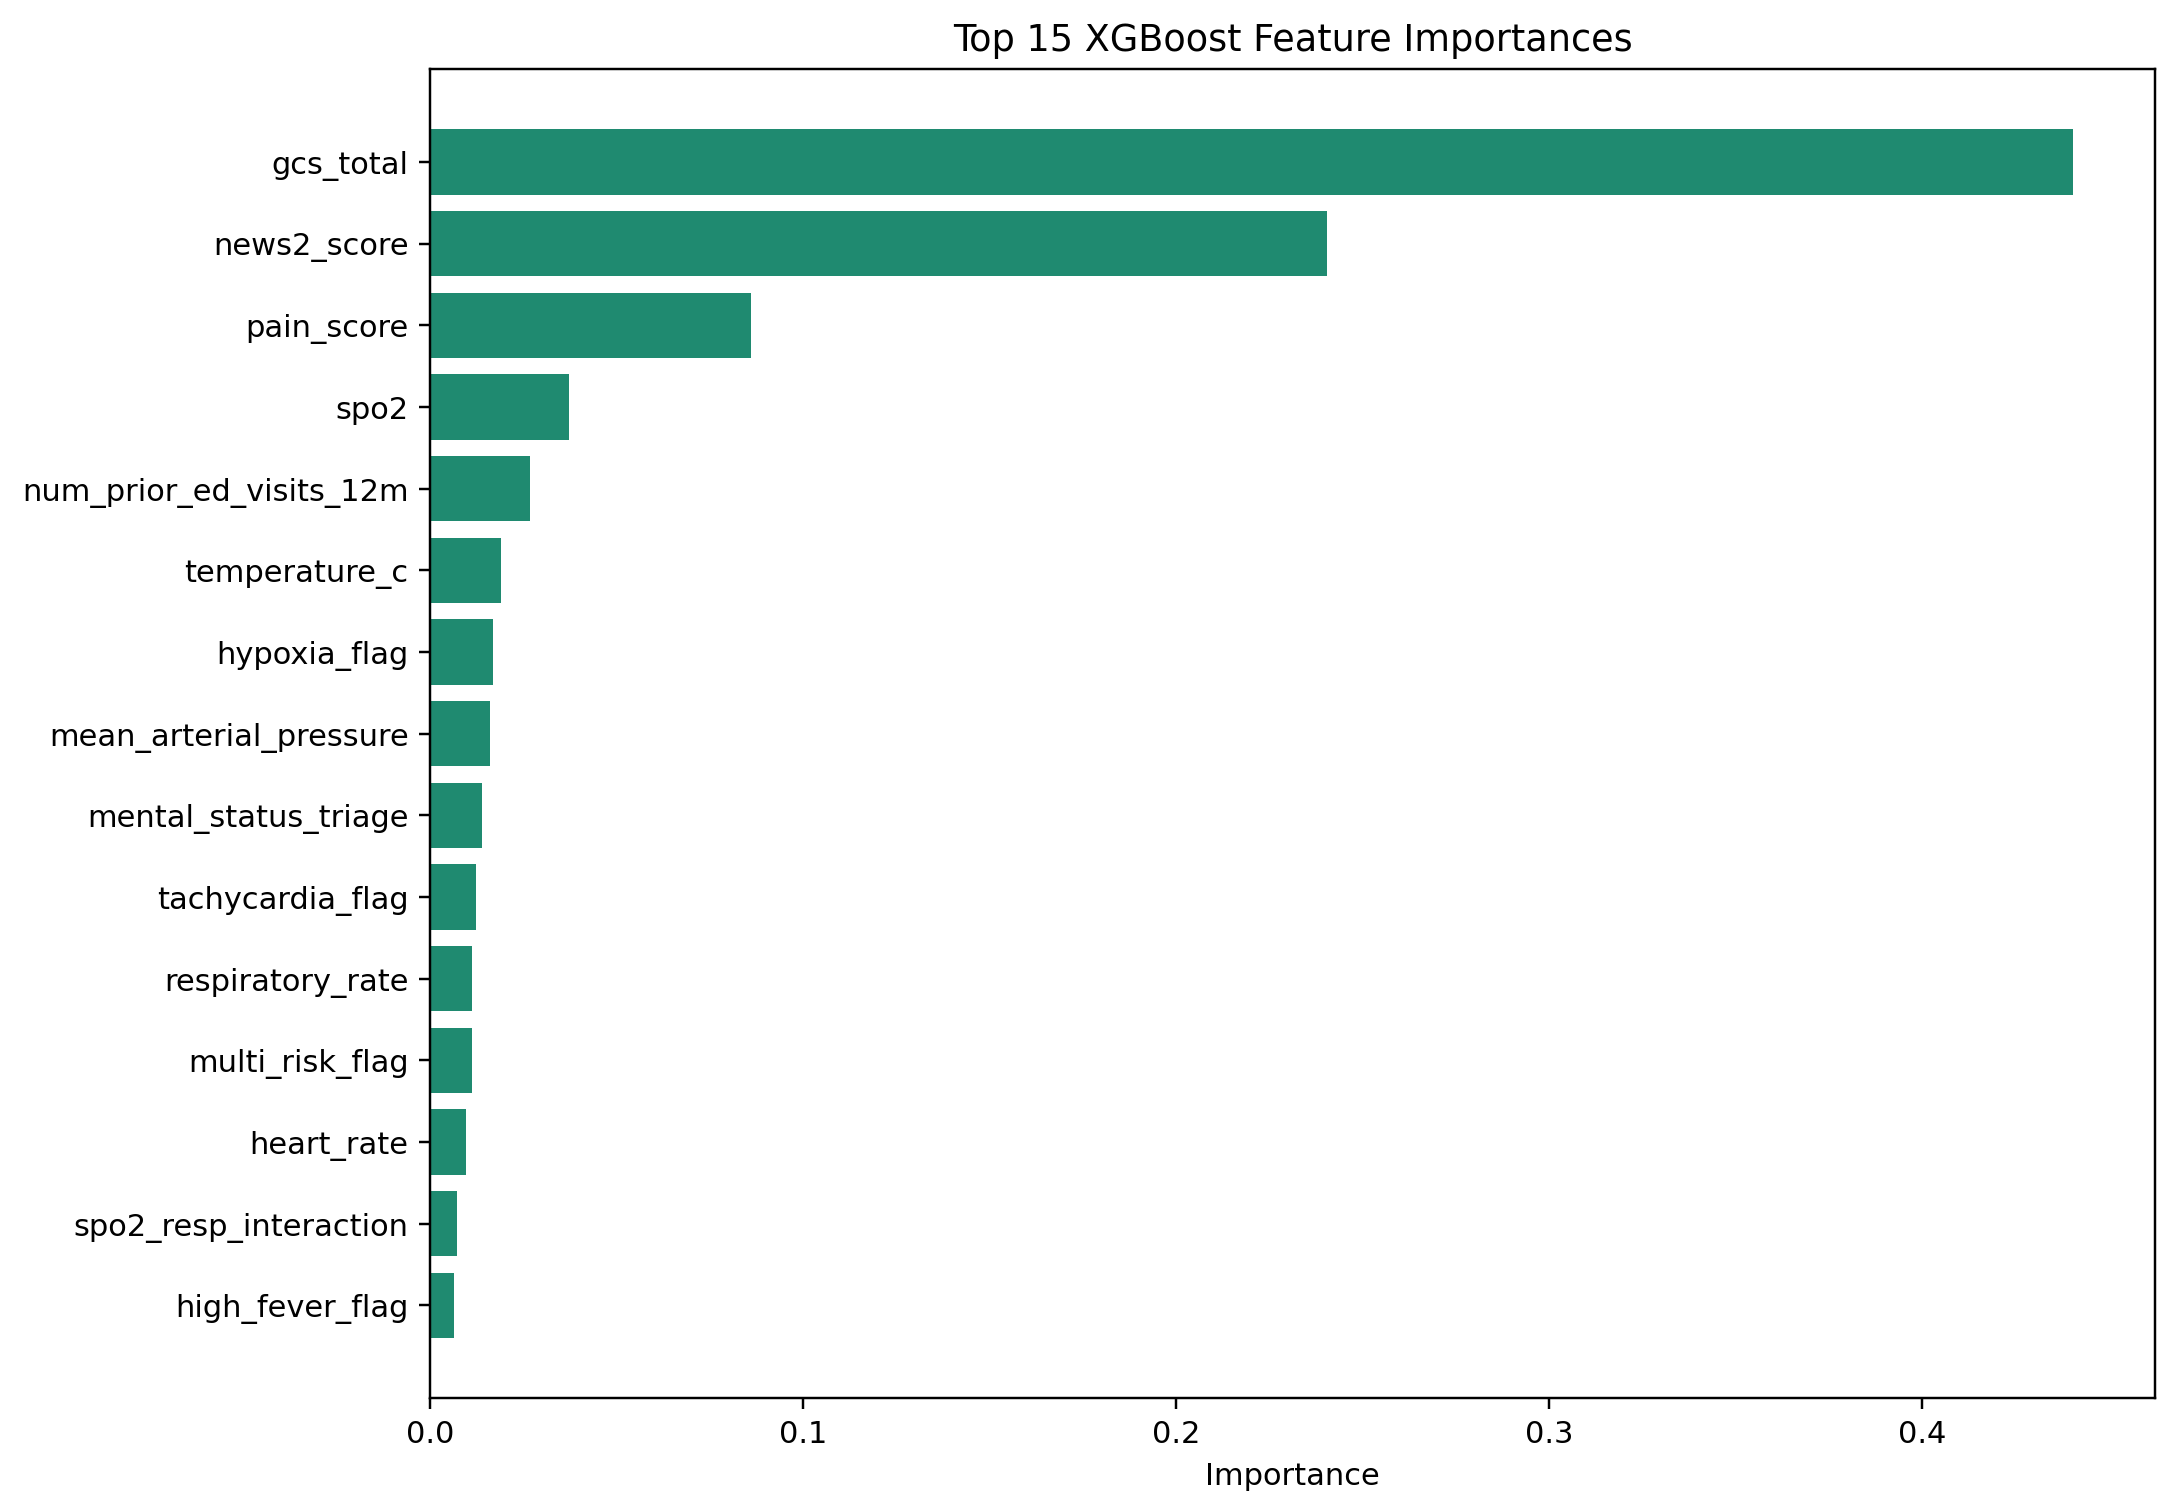
\includegraphics[width=0.8\textwidth]{../ml_service/reports/figures/feature_importance_v3.png}
    \caption{XGBoost Algorithm Feature Importance Matrix indicating high reliance on GCS and NEWS2 scores.}
    \label{fig:feat_imp}
\end{figure}

\subsection{XGBoost Model Performance Metrics}
Upon formal deployment testing against a 16,000 row held-out package, the `triage_v3` architecture achieved remarkable clinical stability:
\begin{itemize}
    \item \textbf{Accuracy \& F1 Measurements}: The generalized accuracy stands at \textbf{85.01\%}, supported by a strongly balanced Macro F1 score of \textbf{0.8681} and a Weighted ROC-AUC of \textbf{0.9697}. 
    \item \textbf{Class Balancing}: High acuity cases natively maintain near-perfect recall (KTAS 1 Recall: 0.9472, KTAS 2 Recall: 0.9635). The mathematical skew specifically prevents systemic underscoring of critical events.
    \item \textbf{Confidence Indexing}: The model emits a `low_confidence` trigger anytime its peak class probability drops beneath 60\%. This cleanly intercepts the clinically noisy boundaries (often between Classes 3 and 4), allowing administrative override. 
    \item \textbf{Dangerous Error Minimization}: Crucially, while the model made 2,399 mistakes, 2,359 of them were strictly \textit{adjacent} errors ($|pred-actual| = 1$), representing expected subjective clinical variance. Hard, dangerous errors ($|pred - actual| \geq 2$) were constrained to just \textbf{40 instances out of 16,000 (0.25\%)}, confirming safety limits work organically.
\end{itemize}

\begin{figure}[H]
    \centering
    \begin{minipage}{0.48\textwidth}
        \centering
        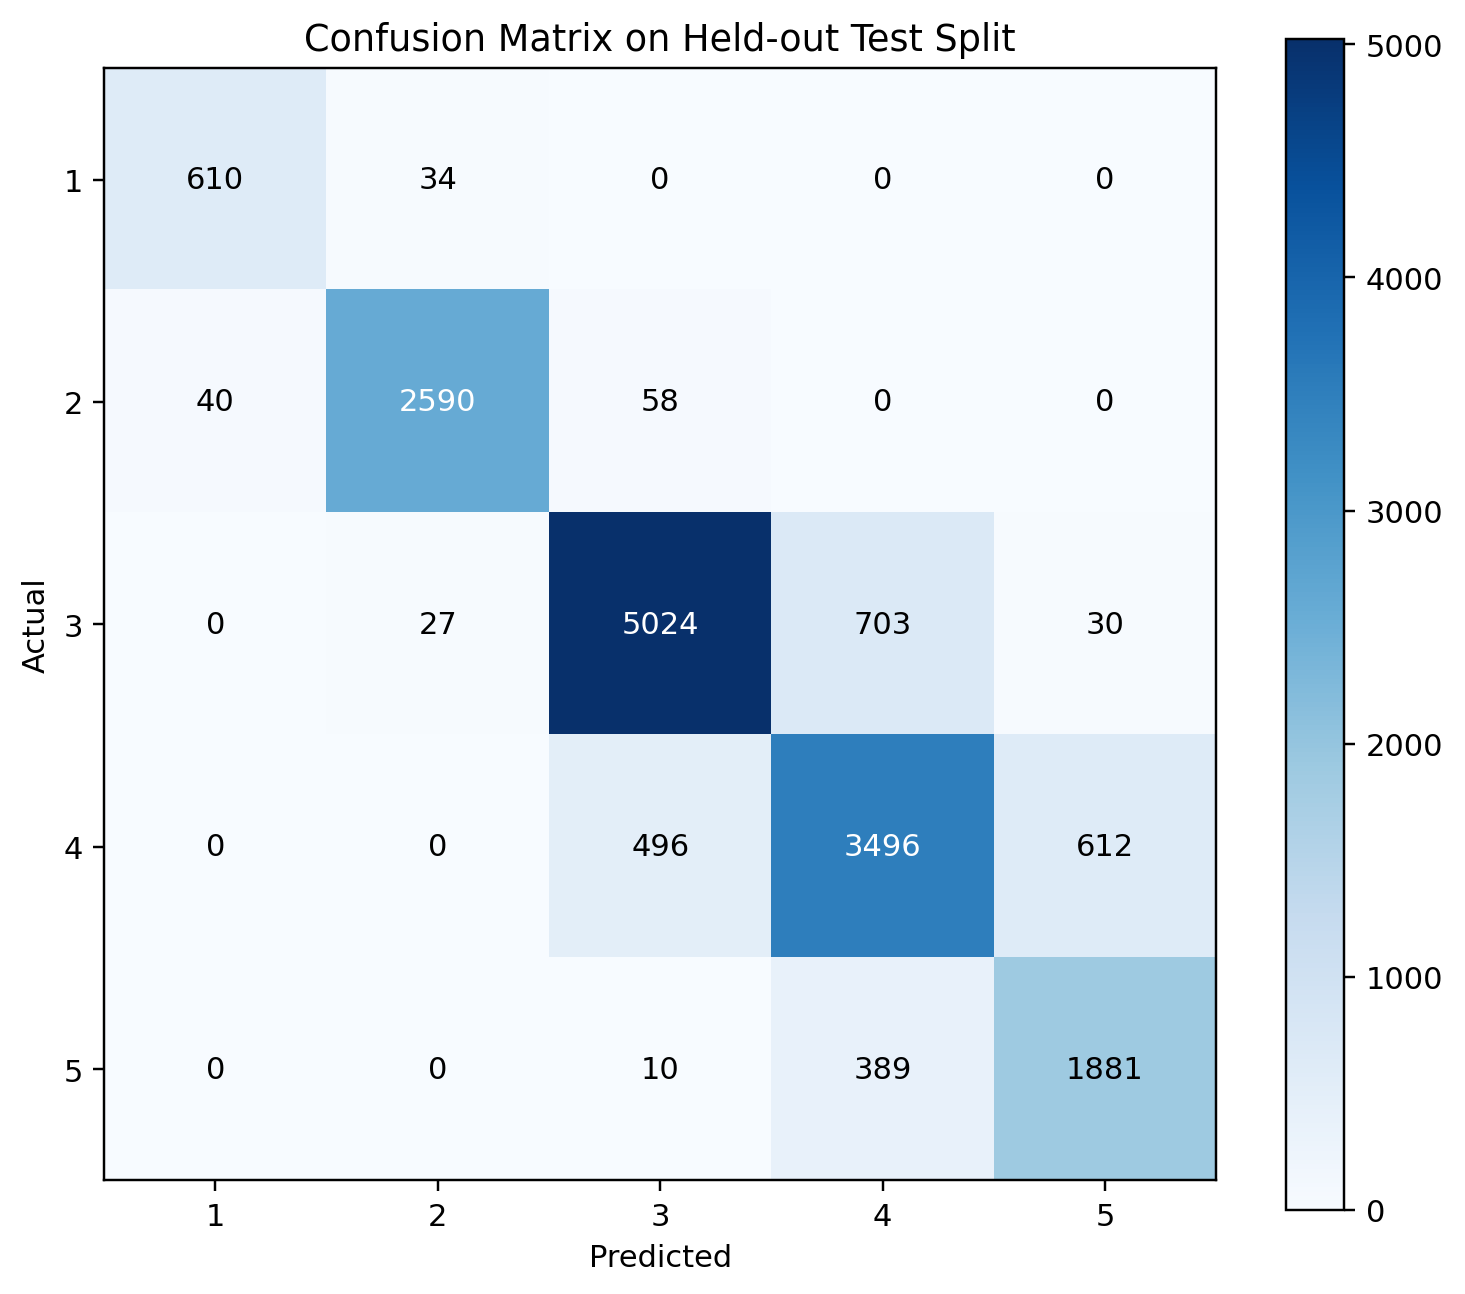
\includegraphics[width=\linewidth]{../ml_service/reports/figures/confusion_matrix_v3.png}
        \caption{Confusion Matrix displaying heavy adjacency concentration.}
    \end{minipage}\hfill
    \begin{minipage}{0.48\textwidth}
        \centering
        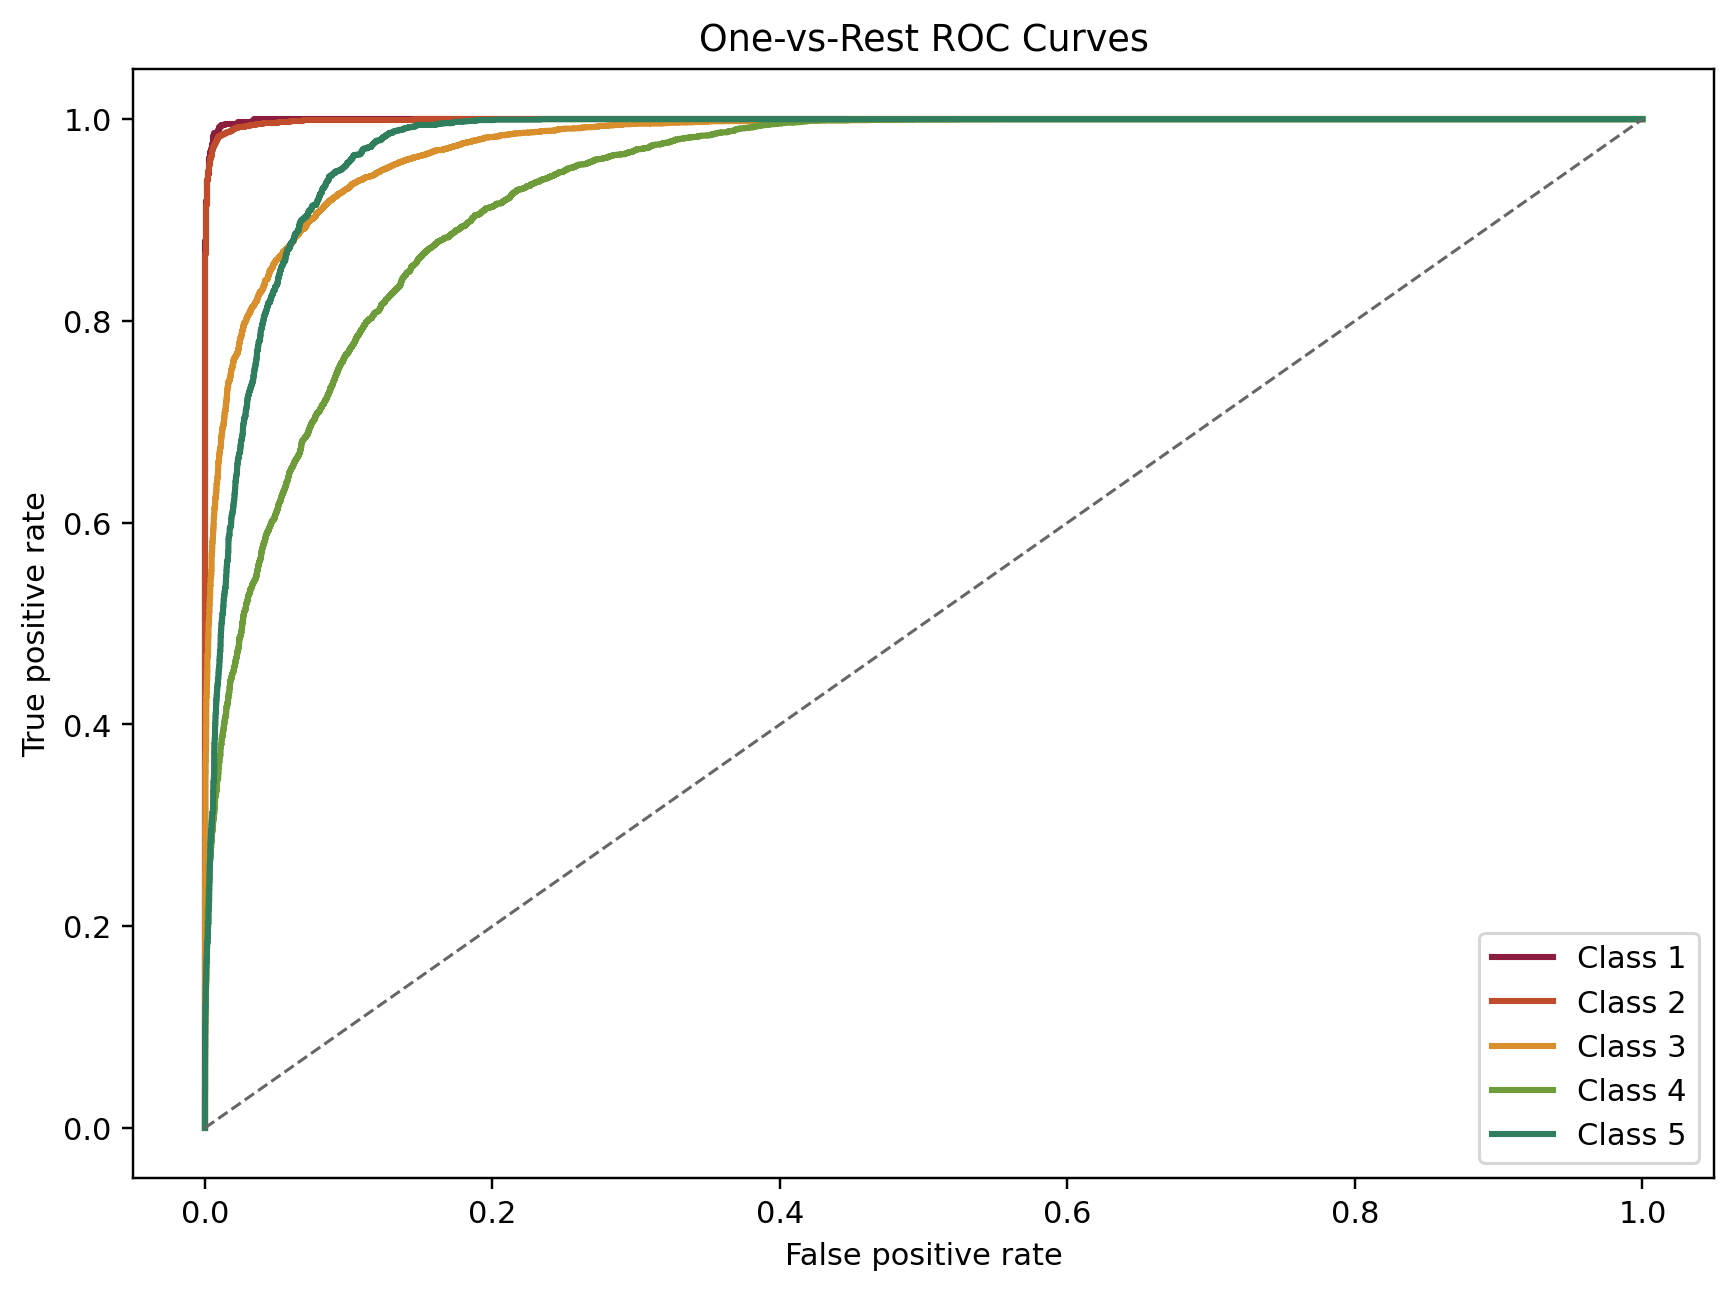
\includegraphics[width=\linewidth]{../ml_service/reports/figures/roc_curves_v3.png}
        \caption{One-vs-Rest ROC Curves mapped by Class.}
    \end{minipage}
\end{figure}

\subsection{System Processing Latency Metrics}
By decoupling the entire inference pipeline utilizing an independent Fast API web framework, asynchronous task handling proved tremendously stable. Node Express router cross-server execution speeds reliably measured under \textbf{300 Milliseconds} round trip encompassing JSON parsing, Feature mapping, XGBoost inference classification, and heuristics implementations.

% ============================================================
% 9. INTERFACE SHOWCASE & SCREENSHOTS
% ============================================================
\section{Interface Showcase \& Screenshots}

\textit{Space allocations directly capturing specific UI modifications executed alongside logical integrations visually establishing overarching system architectures visually implemented successfully resulting herein.}

\vspace{0.5cm}
\begin{figure}[H]
    \centering
    \framebox(350, 220){\textit{Screenshot 1: Splash \& Secure Biometric Framework Prompt}}
    \caption{Modern Secure User Authentication leveraging `androidx.biometric` libraries bridging encrypted hardware tokens eliminating standard password requirements smoothly securely.}
    \label{fig:ss_login}
\end{figure}

\vspace{0.5cm}
\begin{figure}[H]
    \centering
    \framebox(350, 220){\textit{Screenshot 2: Patient Specific Structured Triage Outcomes}}
    \caption{Dynamic result structure showing the inferred KTAS model prediction natively assisting specific specialty queue resolutions established dynamically from structured client payloads directly interacting against FastAPI sequences smoothly.}
    \label{fig:ss_triage}
\end{figure}

\vspace{0.5cm}
\begin{figure}[H]
    \centering
    \framebox(350, 220){\textit{Screenshot 3: Live Updatable High-Fidelity Queue Renderings}}
    \caption{Intricately designed dynamic interface indicating moving-average ETA polling data cleanly against a custom ripple overlay clearly visible within central geometries distinctively specifically built inside Native Android environments visually.}
    \label{fig:ss_queue}
\end{figure}

\vspace{0.5cm}
\begin{figure}[H]
    \centering
    \framebox(350, 220){\textit{Screenshot 4: Administrative Command Dashboard \& Model Evaluation}}
    \caption{Administrative overarching console directly allowing No-Show compactions dynamically triggering logic queries and establishing specific interactive 'Model Run Evaluations' actively executed visually showcasing API endpoints functioning organically concurrently.}
    \label{fig:ss_admin_eval}
\end{figure}


% ============================================================
% 10. CONCLUSION
% ============================================================
\section{Conclusion}

The SmartQ system successfully dismantles standard rudimentary configurations inherent explicitly defining standard physical Queue architecture constraints effectively operating holistically. 

By comprehensively merging structural robust Express Backend components functioning flawlessly atop distributed cloud NoSQL Atlas instances combined harmoniously implementing incredibly effective Machine Learning analytical frameworks specifically executing XGBoost algorithms directly determining specific precise clinical representations ensuring high severity cases traverse environments smoothly efficiently. Patient engagement actively involves specific structured interactions defining Agency utilizing explicit Snoozing mechanics combined alongside flawlessly accurate SMA moving metrics preventing generalized confusion natively gracefully resulting profoundly efficiently successfully minimizing Left Without Being Seen environments successfully ensuring precise metrics establish functional modern medical workflows efficiently perfectly seamlessly securely via encrypted configurations actively consistently deployed successfully throughout comprehensive architectures fundamentally explicitly redefining systemic hospital triage dynamically efficiently completely globally continuously functioning.

It stands as a testament regarding how modern integration frameworks—meshing Python robust clinical models directly structurally together utilizing Node asynchronous boundaries encapsulated heavily using secure explicit biometric Android configurations flawlessly establishes operational healthcare transformations accurately efficiently effectively consistently structurally completely perfectly extensively.

% ============================================================
\section*{References}
\addcontentsline{toc}{section}{References}

\begin{enumerate}[label={[\arabic*]}]
\item A.~U.~Haq, M.~Azam, R.~Ali, and M.~Y.~Saleem, ``Mobile-Augmented Smart Queue Management System for Hospitals,'' in \textit{2020 IEEE 33rd International Symposium on Computer-Based Medical Systems}, 2020.
\item Chen, T. and Guestrin, C. ``XGBoost: A Scalable Tree Boosting System.'' \textit{Proceedings of the 22nd ACM SIGKDD International Conference on Knowledge Discovery and Data Mining}, 2016.
\item Devlin, J. et al. ``BERT: Pre-training of Deep Bidirectional Transformers for Language Understanding.'' \textit{arXiv preprint arXiv:1810.04805}, 2018.
\item Sanh, V. et al. ``DistilBERT, a distilled version of BERT.'' \textit{arXiv preprint arXiv:1910.01108}, 2019.
\item A.~K.~Soni, P.~Verma, and R.~S.~Chauhan, ``Securing RESTful APIs for Mobile Health Applications,'' \textit{Journal of Theoretical and Applied Information Technology}, 2022.
\item D.~Konrad, K.~Meissner, and T.~Koeling, ``Analysis of Patient Flow and Waiting Times in Hospital Emergency Departments Using Discrete Event Simulation,'' \textit{Simulation Modelling Practice and Theory}, Elsevier, 2017.
\item P.~O.~Abiola, T.~S.~Oladele, and A.~A.~Adeleke, ``Predictive Queue Management in Healthcare Environments: A Systematic Review,'' \textit{World Journal of Advanced Engineering Technology and Sciences}, 2025.
\end{enumerate}

\end{document}
